\ccUserChapter{Kinetic Data Structures\label{chapter-kds}}
\ccChapterAuthor{Daniel Russel} 

%\chapter{Kinetic Data Structures}



%
\begin{ccPkgDescription}{3D Triangulations}
\ccPkgSummary{
This package  allows to build and handle
triangulations for point sets in three dimensions.
Any CGAL  triangulation covers the convex hull of its
vertices. Triangulations are build incrementally 
and can be modified by insertion or removal of vertices. 
They offer point location facilities.

The package provides plain triangulation (whose faces
depends on the  insertion order of the vertices) and
Delaunay triangulations.  Regular triangulations are
also provided for sets of weighted points.
Delaunay and regular
triangulations offer nearest neighbor queries
and primitives to build the dual Voronoi and power diagrams.}

%\ccPkgDependsOn{}
\ccPkgMaturity{Introduced in \cgal\ 3.1}

\end{ccPkgDescription}


\minitoc


\ccDefGlobalScope{CGAL::}

\def\note#1{$\langle\langle${\bf #1}$\rangle\rangle$}
%\message{Remove note before final version!}
%\def{\th}{^{\rm th}}

% space tweaks
%\addtolength{\parskip}{-1pt}

%\section{Todo}

\subsection{General thoughts}

\begin{itemize}

\item I like the idea of changing MovingObjectTable to ActiveObjectTable. Not sure if Notifying\_table should follow suit. 

\item Regular triangulation 3 is not entirely working.

\item I reorganized out of existance my 3D demos.

\item The other trajectory modification events need to be documented

\item There is no testing of the Delaunay 3 Visitor class. 

\item The architeture figure goes to the end for some reason. 

\end{itemize}

%%% Local Variables: 
%%% mode: latex
%%% TeX-master: t
%%% End: 


Lets say you want to maintain a sorted list of items (each item is
associate with a real number key). You can imagine placing each of the
items on the point on the real line corresponding to its key. Now, let
the key for each item change continuously (i.e. no jumps are allowed).
As long as no to (consecutive) items cross, the sorted order is
intact. When two cross, they need to be exchanged in the list and then
the sorted order is once again correct. This is a trivial example of a
kinetic data structure. The key observation is that the combinatorial
structure which is maintained changes at discrete times (events) even
though the basic building blocks are changing continuously.

This chapter describes a number of such kinetic data structures
implemented using the Kinetic framework described in
Chapter~\ref{chapter-kinetic}. We first, in
Section~\ref{sec:kds_intro} introduce kinetic data structures and
sweepline algorithms. This section can be skipped if the reader is
already familiar with the area. The next sections,
Section~\ref{sec:kds_terms} and Section~\ref{sec:kds_overview} introduces
the terms and gives an overview of the framework. They are recommended
reading for all readers, even if you are just using provided kinetic
data structures. We then present kinetic data structures for Delaunay
triangulations in two and three dimensions in
Section~\ref{sec:kds_provided_kdss}.

%%%%%%%%%%%%%%%%%%%%%%%%%%%%%%%%%%%%%%%%%%%%%%%%%%%%%%%%%%%%%%%%%%%%
\section{An Overview of Kinetic Data Structures and Sweep Algorithms\label{sec:kds_intro}}

%%%%%%%%%%%%%%%%%%%%%%%%%%%%%%%%%%%%%%%%%%%%%%%%%%%%%%%%%%%%%%%%%%%%


%\subsection{Kinetic Data Structures}
Kinetic data structures were first introduced in by Basch et.\ al.\ in
1997~\cite{cgal:bgh-dsmd-97}.  The idea stems from the observation that
most, if not all, computational geometry structures are built using
{\em predicates} --- functions on quantities defining the geometric
input (e.g.\ point coordinates), which return a discrete set of
values. Many predicates reduce to determining the sign of a polynomial
on the defining parameters of the primitive objects. For example, to
test whether a point lies above or below a plane we compute the dot
product of the point with the normal of the plane and subtract the
plane's offset along the normal. If the result is positive, the point
is above the plane, zero on the plane, negative below. The validity of
many combinatorial structures built on top of geometric primitives can
be verified by checking a finite number of predicates of the geometric
primitives.  These predicates, which collectively certify the
correctness of the structure, are called {\em certificates}.  For a
Delaunay triangulation in three dimensions, for example, the
certificates are one \ccc{InCircle} test per facet of the
triangulation, plus a point plane orientation test for each facet or
edge of the convex hull.

The kinetic data structures approach is built on top of this view of
computational geometry. Let the geometric primitives move by replacing
each of their defining quantities with a function of time (generally a
polynomial). As time advances, the primitives trace out paths in
space called {\em trajectories}. The values of the polynomial
functions of the defining quantities used to evaluate the predicates now
also become functions of time. We call these functions
{\em certificate functions}. Typically, a geometric structure is valid when
all predicates have a specific non-zero sign. In the kinetic setting,
as long as the certificate functions maintain the correct sign as time varies,
the corresponding predicates do not change values,
and the original data structure remains correct. However, if
one of the certificate functions changes sign, the original structure
must be updated, as well as the set of certificate functions that
verify it.  We call such occurrences {\em events}.

Maintaining a kinetic data structure is then a matter of determining
which certificate function changes sign next, i.e.\ determining which
certificate function has the first real root that is greater than the
current time, and then updating the structure and the set of
certificate functions. In addition, the trajectories of primitives are
allowed to change at any time, although $C^0$-continuity of the
trajectories must be maintained.  When a trajectory update occurs for
a geometric primitive, all certificates involving that primitive must
be updated.  We call the collection of kinetic data structures,
primitives, event queue and other support structures a
{\em simulation}.

Sweepline algorithms for computing arrangements in $d$ dimensions
easily map on to kinetic data structures by taking one of the
coordinates of the ambient space as the time variable. The kinetic
data structure then maintains the arrangement of a set of objects
defined by the intersection of a hyperplane of dimension $d-1$ with
the objects whose arrangement is being computed. 


Time is one of the central concepts in a kinetic simulation.  Just as
static geometric data structures divide the continuous space of all
possible inputs (as defined by sets of coordinates) into a discrete
set of combinatorial structures, kinetic data structures divide the
continuous time domain into a set of disjoint intervals. In each
interval the combinatorial structure does not change, so, in terms of
the combinatorial structure, all times in the interval are equivalent.
We capitalize on this equivalence in the framework in order to
simplify computations. If the primitives move on polynomial
trajectories and the certificates are polynomials in the coordinates,
then events occur at real roots of polynomials of time. Real numbers,
which define the endpoints of the interval, are more expensive to
compute with than rational numbers, so performing computations at a
rational number inside the interval is preferable whenever
possible. See Section~\ref{sec:kds_instantaneous_kernel} for an example of
where this equivalence is exploited.

%%%%%%%%%%%%%%%%%%%%%%%%%%%%%%%%%%%%%%%%%%%%%%%%%%%%%%%%%%%%%%%%%%%%
\subsection{Terms Used\label{sec:kds_terms}}

%%%%%%%%%%%%%%%%%%%%%%%%%%%%%%%%%%%%%%%%%%%%%%%%%%%%%%%%%%%%%%%%%%%%

\begin{description}
\item[primitive] The basic geometric types, e.g., the points of a
  triangulation. A primitive has a set of {\em coordinates}.
\item[combinatorial structure] A structure built on top of the
  primitives. The structure does not depend directly on the
  coordinates of the primitives, only on relationships between them.
\item[trajectory] The path traced out by a primitive as time passes.
  In other words how the coordinates of a primitive change with time.
\item[snapshot] The position of all the primitives at a particular
  moment in time.
\item[static] Having to do with geometric data structures on
  non-moving primitives.
\item[predicate] A function which takes the coordinates of several
  primitives from a snapshot as input and produces one of a discrete
  set of outputs.
\item[certificate] One of a set of predicates which, when all having
  the correct values, ensure that the combinatorial structure is
  correct.
\item[certificate function] A function of time which is positive when
  the corresponding certificate has the correct value. When the
  certificate function changes sign, the combinatorial structure needs
  to be updated.
\item[event] When a certificate function changes sign and the
  combinatorial structure needs to be updated.
\end{description}


\section{An Overview of the Kinetic Framework\label{sec:kds_overview}}

The provided kinetic data structures are implemented on top of the
Kinetic framework presented in Chapter~\ref{chapter-kinetic}. It is
not necessary to know the details of the framework, but some
familiarity is useful. Here we presented a quick overview of the
framework.

The framework is structured around five main concepts. See
Figure~\ref{fig:kds_uml_usage} for a schematic of how a kinetic data
structure interacts with the various parts. The main concepts are
 
% MK:: why is there a + before less_x_1_object() ?
% Another thing is that I am not really sure that we really want this
% figure to appear here. I prefer to have it at the end as it was before.
% I leave it up to you to decide this.


\begin{itemize}

\item the \ccc{Kinetic::Simulator}. Models of this concept process events in
  the correct order and audit kinetic data structures. There should be
  one instance of a model of this concept per simulation.
\item the \ccc{Kinetic::Kernel}. The structure of a
  \ccc{Kinetic::Kernel} is analogous to the static \cgal\ (i.e.,
  non-kinetic) kernels in that it defines a set of primitives and
  functors which generate certificates from the primitives.
\item the \ccc{Kinetic::ActiveObjectsTable}. Models of this concept hold a
  collection of kinetic primitives in a centralized manner. This
  structure centralizes management of the primitives in order to
  properly disseminate notifications when trajectories change, new
  primitives are added or primitives are deleted.
  There is generally one instance of a model of this concept per simulation.
\item the \ccc{Kinetic::InstantaneousKernel}. Models of this concept allow
  existing non-kinetic \cgal\ data structures to be used on a snapshot
  of kinetic data. As a result, pre-existing static structures can be
  used to initialize and audit kinetic data structures.
\item the \ccc{Kinetic::FunctionKernel}. This concept is the computational
  kernel of our framework.  Models of this concept are responsible for
  representing, generating and manipulating the motional and
  certificate functions and their roots. It is this concept that
  provides the kinetic data structures framework with the necessary
  algebraic operations for manipulating event times. The
  \ccc{Kinetic::FunctionKernel} is discussed in detail in Section
  \ref{sec:kds_algebraic_kernel}.
\end{itemize}

\begin{figure}
\begin{ccTexOnly}
\begin{center}
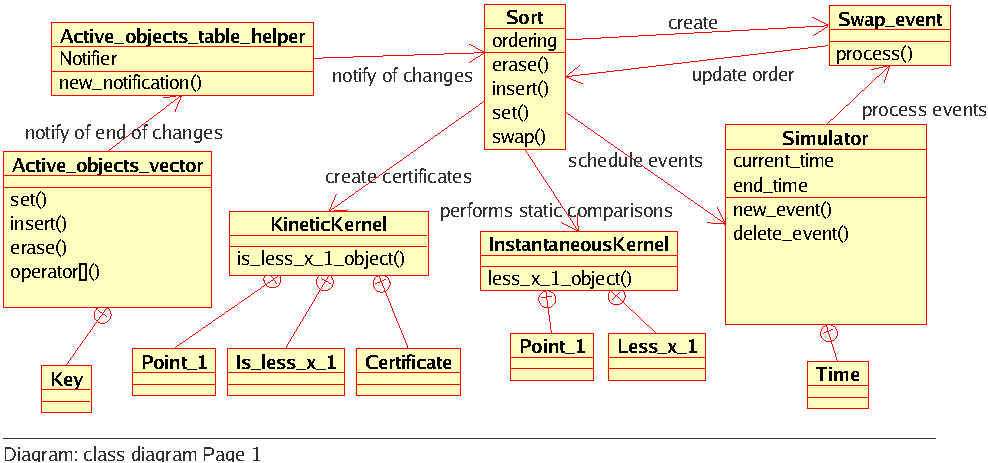
\includegraphics[scale=.8,viewport=0 18 470 250, clip]{Kinetic_data_structures/sort_usage_pct}
\end{center}
\end{ccTexOnly}
\begin{ccHtmlOnly}
<img src="./sort_usage_pct.gif" align=middle alt="Sort Usage"><br>
\end{ccHtmlOnly}
\caption{\label{fig:kds_uml_usage} The figure shows the interaction between
  the \ccc{Kinetic::Sort<Traits, Visitor>} kinetic data structure and
  the various pieces of our package.  Other, more complicated, kinetic
  data structures will also use the \ccc{Kinetic::InstantaneousKernel} in order
  to insert/remove geometric primitives and audit
  themselves. \ccc{Kinetic::Sort<Traits, Visitor>} uses the sorting
  functionality in the {\sc Stl} instead.}
\end{figure}

For simplicity, we added an additional concept, that of
\ccc{Kinetic::SimulationTraits}, which wraps together a particular set of
choices for the above concepts and is responsible for creating
instances of each of the models. As a user of existing kinetic data
structures, this is the only framework object you will have to
create. The addition of this concept reduces the choices the user has
to make to picking the dimension of the ambient space and choosing
between exact and inexact computations. The model of
\ccc{Kinetic::SimulationTraits} creates an instance each of the
\ccc{Kinetic::Simulator} and \ccc{Kinetic::ActiveObjectsTable}. Handles for
these instances as well as instances of the \ccc{Kinetic::Kernel}
and \ccc{Kinetic::InstantaneousKernel} can be requested from the simulation
traits class. Both the \ccc{Kinetic::Kernel} and the
\ccc{Kinetic::Simulator} use the \ccc{Kinetic::FunctionKernel},
 the former to find certificate failure times and the later to operate
on them. For technical reasons, each supplied model of
\ccc{Kinetic::SimulationTraits} also picks out a particular type of
kinetic primitive which will be used by the kinetic data structures.


% Both the \object{KineticKernel}
%and the \object{Simulator} query the \object{FunctionKernel} for
%constructing certificate functions, as well as getting their failure
%times.





\section{Using Kinetic Data Structures\label{sec:kds_provided_kdss}}


There are five provided kinetic data structures. They are
\begin{description}
\item[\ccc{Kinetic::Sort<Traits, Visitor>}] maintain a list of points
sorted by x-coordinate.
\item[\ccc{Kinetic::Delaunay_triangulation_2<Traits, Visitor,
    Triangulation>}] maintain the Delaunay triangulation of a set of
  two dimensional points
\item[\ccc{Kinetic::Delaunay_triangulation_3<Traits,Visitor,
    Triangulation>}] maintain the Delaunay triangulation of a set of
  three dimensional points.
\item[\ccc{Kinetic::Regular_triangulation_3<Traits, Visitor,
Triangulation>}] maintain the regular triangulation of a set of waiting
three dimensional points.
\item[\ccc{Kinetic::Enclosing_box_2<Traits>},
  \ccc{Kinetic::Enclosing_box_3<Traits>}] restrict points to stay
  within a box by bouncing them off the walls.
\end{description}


\subsection{Two Dimensional Delaunay}
\label{sec:sort_example}

Using a kinetic data structure can be as simple as the following:
\label{fig:sort_program}
\ccIncludeExampleCode{Kinetic_data_structures/sort.C}

In the example, first the Kinetic::SimulationTraits object is chosen
(in this case one that supports exact computations). Then the kinetic
data structure is defined, using the chosen traits object and a
visitor class which logs changes to the sorted list.  Next, instances
of the two are created and a set of points is read from a file. Then,
the simulator is instructed to process all the events until the end of
the simulation.  Finally, a record of what happened is printed to the
terminal.

Several important things happen behind the scenes in this example.
First, the Kinetic::ActiveObjectsTable which holds the moving points
notifies the kinetic data structure that new points have been added to
the simulation. Second, the \ccc{Kinetic::Sort<Traits,Visitor>} kinetic data structure
registers its events with the Kinetic::Simulator by providing a time
and a proxy object. When a particular event occurs, the
Kinetic::Simulator calls a function on the proxy object which in turn
updates the kinetic data structure.

The example illustrates how to monitor the supplied data structures as
they evolve by using a Kinetic::SortVisitor object---a small class whose
methods are called whenever the kinetic data structure changes. Hooks
for such visitor concepts are provided for all of the shipped kinetic
data structures. In the case of kinetic sorting, the visitor's
methods are called every time a new point is inserted in the sorted
list, when one is removed, or when two points are swapped in the
sorted order. 


The visitor concept is quite powerful, allowing us, for example, to
implement a data structure for computing and storing two-dimensional
arrangements of $x$-monotone curves on top of the
\ccc{Kinetic::Sort<Traits, Visitor>} data structure using about 60
lines of code. This sweepline code is presented in
Section~\ref{sec:sweepline_example}.




\subsection{Visualization of Kinetic Data Structures\label{sec:kds_delaunay_2_example}}


The framework includes Qt widgets for displaying kinetic data
structures in two and three dimensions. The following example shows
using the two dimensional widget with a Delaunay triangulation:

\begin{ccExampleCode}
#include <CGAL/Kinetic/Exact_simulation_traits.h>
#include <CGAL/Kinetic/Delaunay_triangulation_2.h>
#include <CGAL/Kinetic/Enclosing_box_2.h>
#include <CGAL/Kinetic/IO/Qt_moving_points_2.h>
#include <CGAL/Kinetic/IO/Qt_triangulation_2.h>
#include <CGAL/Kinetic/IO/Qt_widget_2.h>

int main(int argc, char *argv[]) {
    using namespace CGAL::Kinetic;
    typedef Exact_simulation_traits Traits;
    typedef Delaunay_triangulation_2<Traits> Del_2;
    typedef Enclosing_box_2<Traits> Box_2;
    typedef Qt_widget_2<Traits::Simulator> Qt_widget;
    typedef Qt_moving_points_2<Traits, Qt_gui> Qt_mps;
    typedef Qt_triangulation_2<Del_2, Qt_widget, Qt_mps> Qt_dt2;
    
    // create a simulation traits and add two KDSs:
    // a kinetic Delaunay triangulation and an enclosing box;
    // the moving points bounce against the walls of the enclosing box
    Traits tr;
    Box_2::Handle box = new Box_2(tr);
    Del_2::Handle kdel = new Del_2(tr);

    // register the simulator, set of moving points and
    // Delaunay triangulation with the kinetic Qt widget
    Qt_widget::Handle qt_w = new Qt_widget(argc, argv, tr.simulator_handle());
    Qt_mps::Handle qt_mps = new Qt_mps(qt_w, tr);
    Qt_dt2::Handle qt_dt2 = new Qt_dt2(kdel, qt_w, qt_mps);

    // read the trajectories of the moving points
    //  the simulation traits automatically inserts them in the two KDSs
    // and schedules the appropriate kinetic events; as in the kinetic
    // sorting example this is done with appropriate notifications
    std::ifstream in("data/points_2");    
    in  >> *tr.active_points_2_table_handle();

    // run the interactive kinetic simulation
    return qt_w->begin_event_loop();
};
\end{ccExampleCode}

The example shows how to use a number of additional features of the
framework. First, it shows that two kinetic data structures
(\ccc{Kinetic::Delaunay_triangulation_2<Traits, Triangulation>} and
\ccc{Kinetic::Enclosing_box_2<Traits>}) can coexist on the same set of
points without any extra effort. Both interact with the moving points
through the active objects table, and never need to directly interact
with one another. Second, objects (like
\texttt{qt\_w}, \texttt{qt\_mps} and \texttt{qt\_dt2}) are all stored
by using reference counted handles (\texttt{Object::Handle}). This
allows them to share references to one another without the user having
to worry about memory management and order of deletion.  For example,
the \ccc{Kinetic::Qt_triangulation_2<KineticDelaunay_2, QtWidget_2,
Qt_moving_points_2>} object needs a handle to the kinetic
triangulation, in order to get the structure to display, and a handle
to the \ccc{Active_points_1_table} to get the coordinates of the
points.


Finally, the example shows how to use the graphical interface elements
provided, see Figure~\ref{fig:kds_qtwidget_capture}. Our package includes
\texttt{Qt} widgets for displaying kinetic geometry in two and three
dimensions. In addition to being able to play and pause the
simulation, the user can step through events one at a time and reverse
the simulation to retrace what had happened. The three-dimensional
visualization support is based on the Coin library http://www.coin3d.org.

\begin{figure*}[htb]
\begin{ccTexOnly}
\begin{center}
1.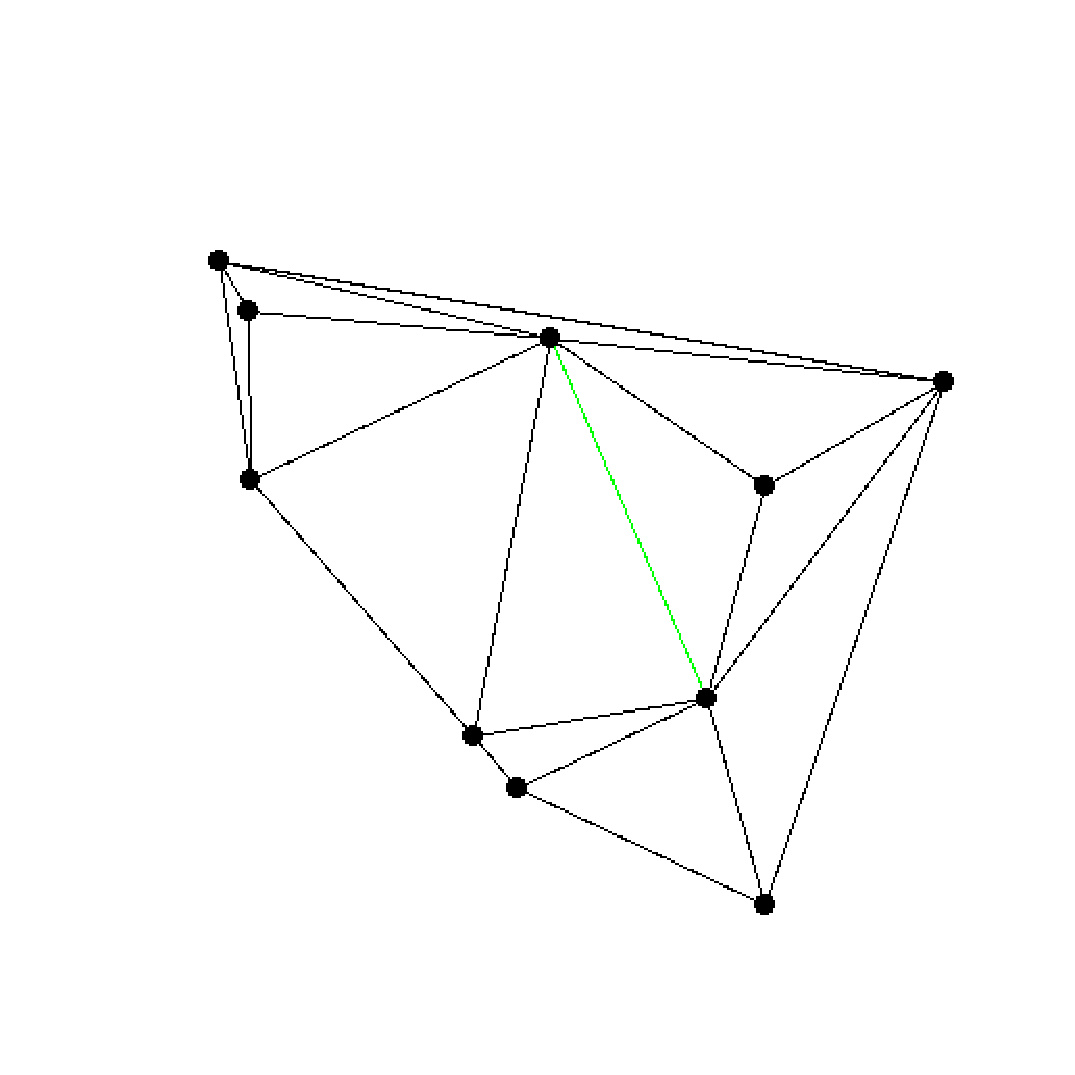
\includegraphics[ scale=.2]{Kinetic_data_structures/delaunay_0} 
2.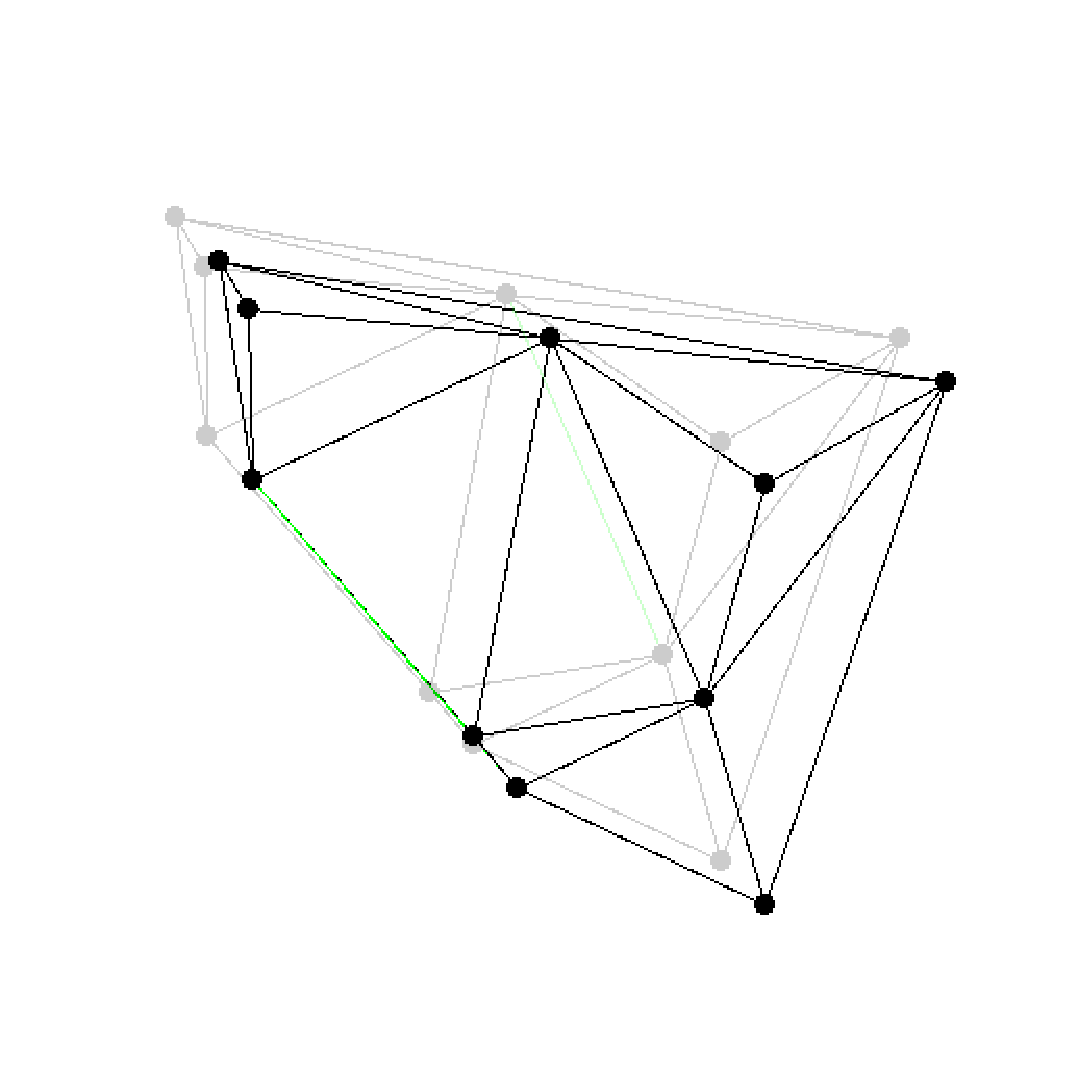
\includegraphics[ scale=.2]{Kinetic_data_structures/delaunay_1}
3.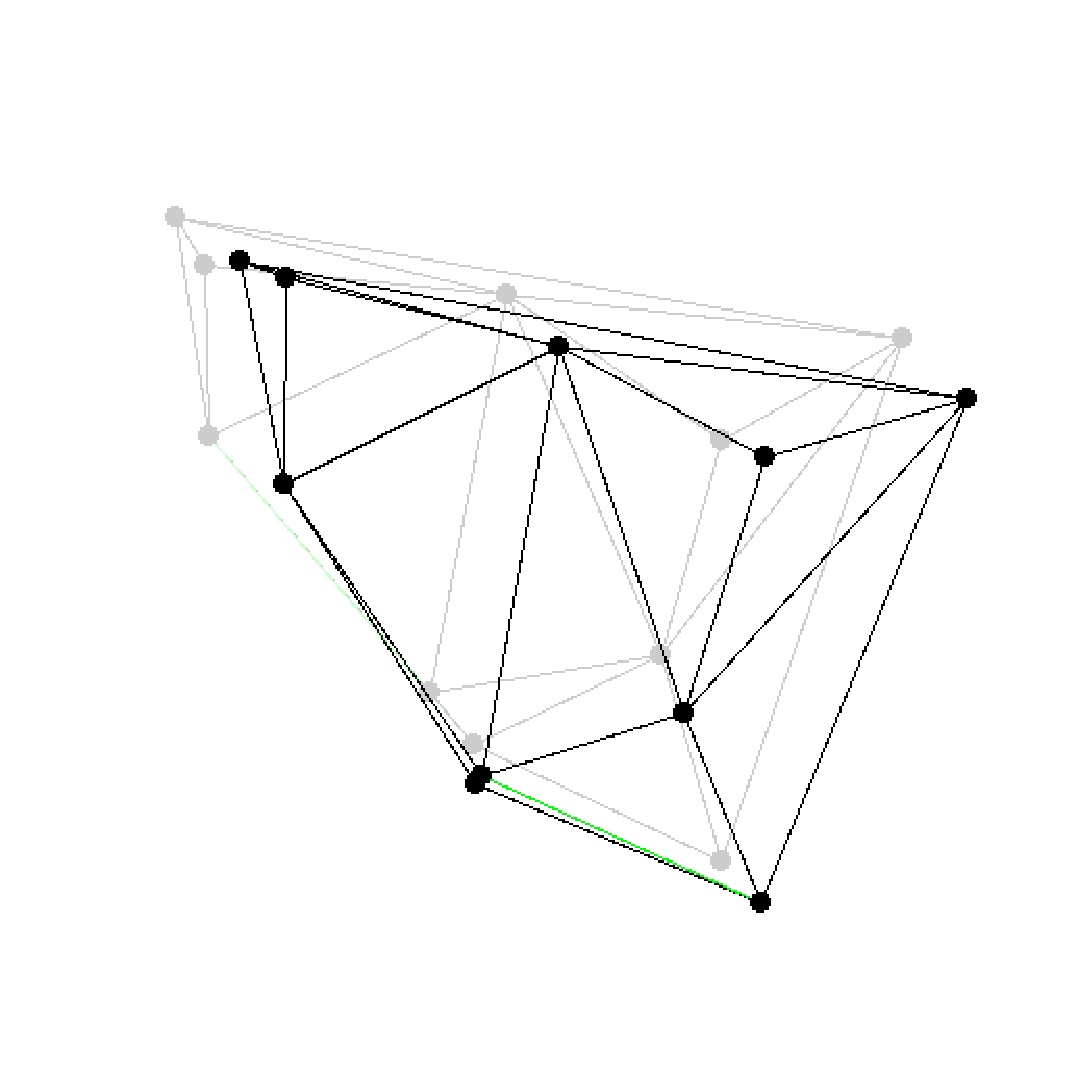
\includegraphics[ scale=.2]{Kinetic_data_structures/delaunay_2}\\
4.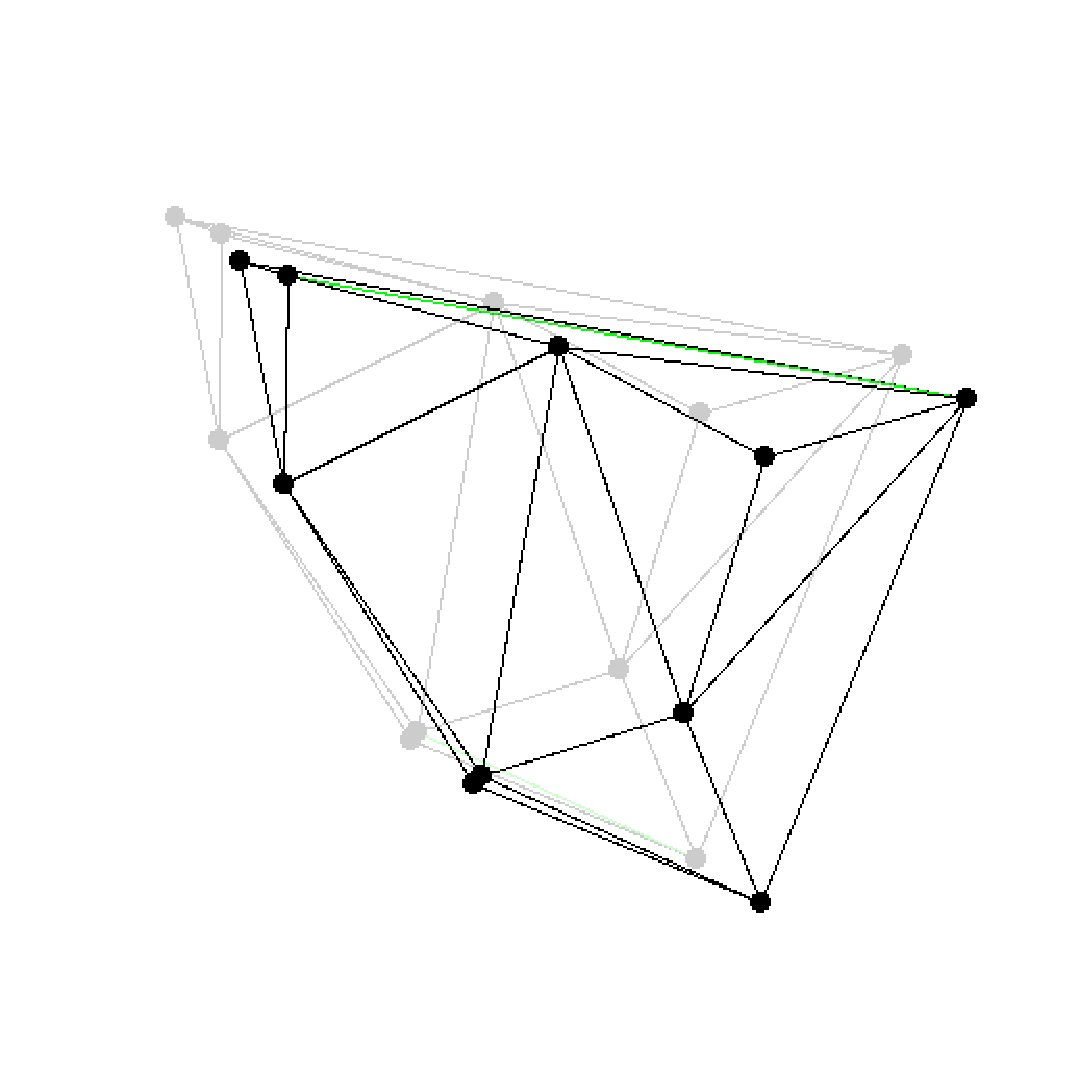
\includegraphics[ scale=.2]{Kinetic_data_structures/delaunay_3}
5.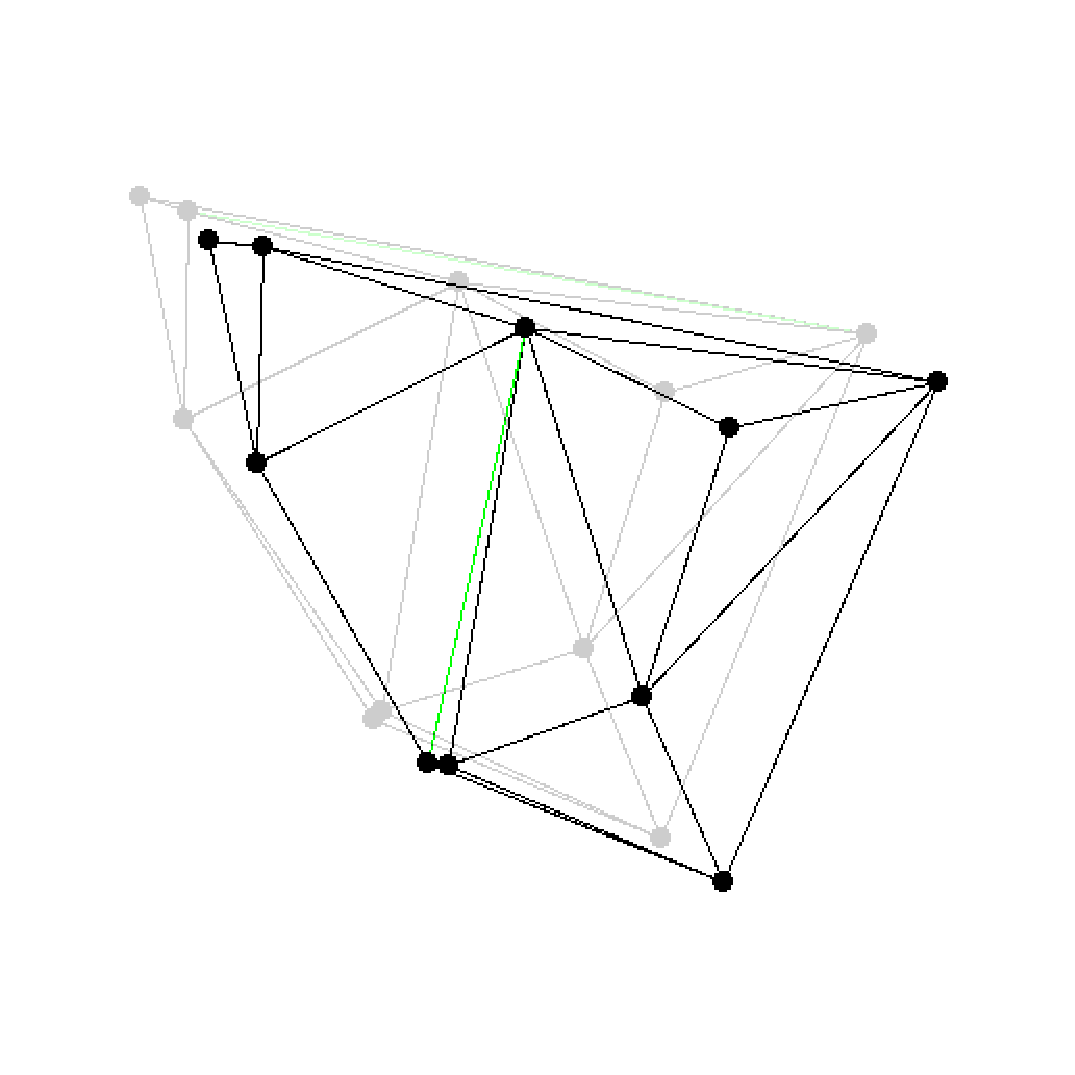
\includegraphics[ scale=.2]{Kinetic_data_structures/delaunay_4}
6.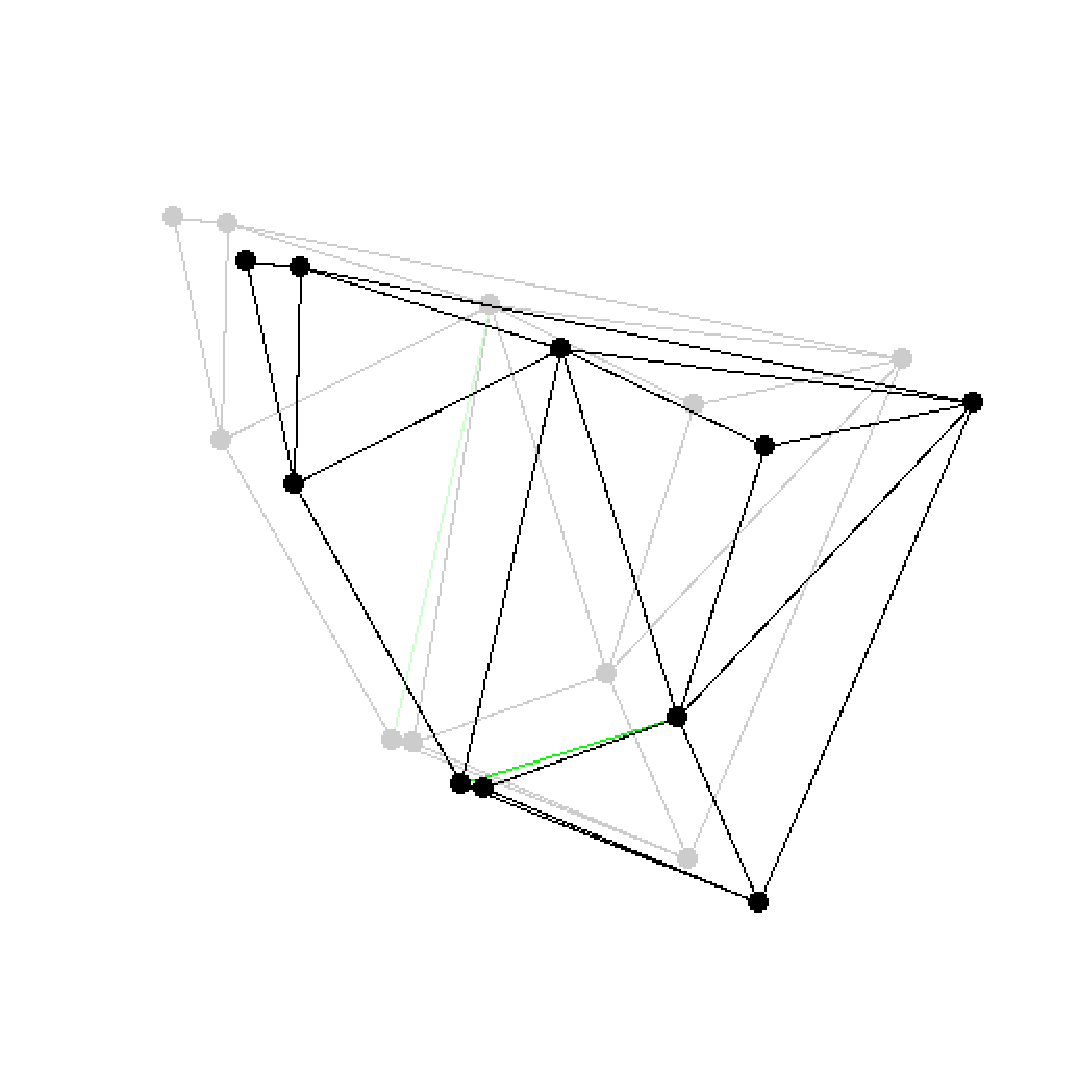
\includegraphics[ scale=.2]{Kinetic_data_structures/delaunay_5}\\
7.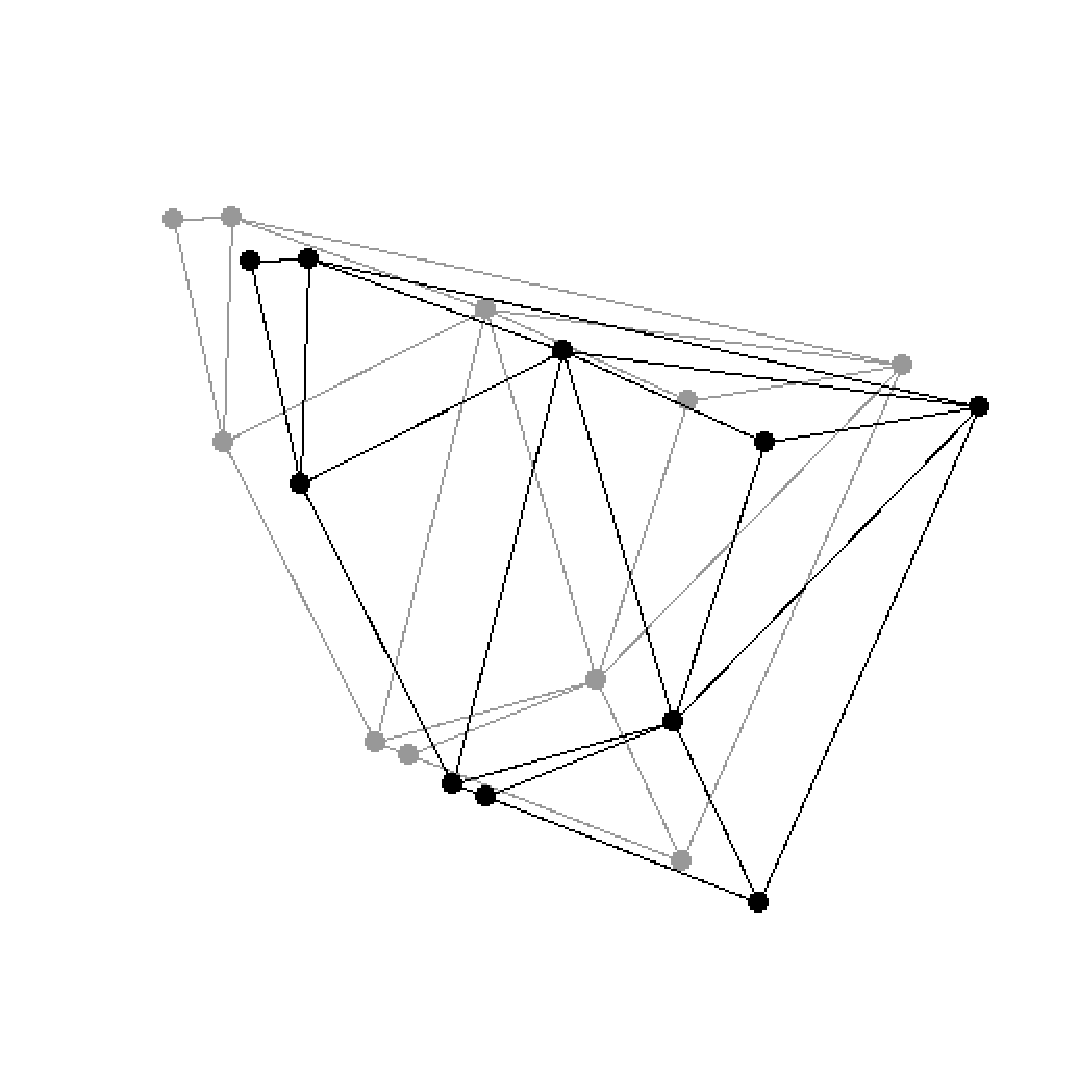
\includegraphics[ scale=.2]{Kinetic_data_structures/delaunay_6}
8.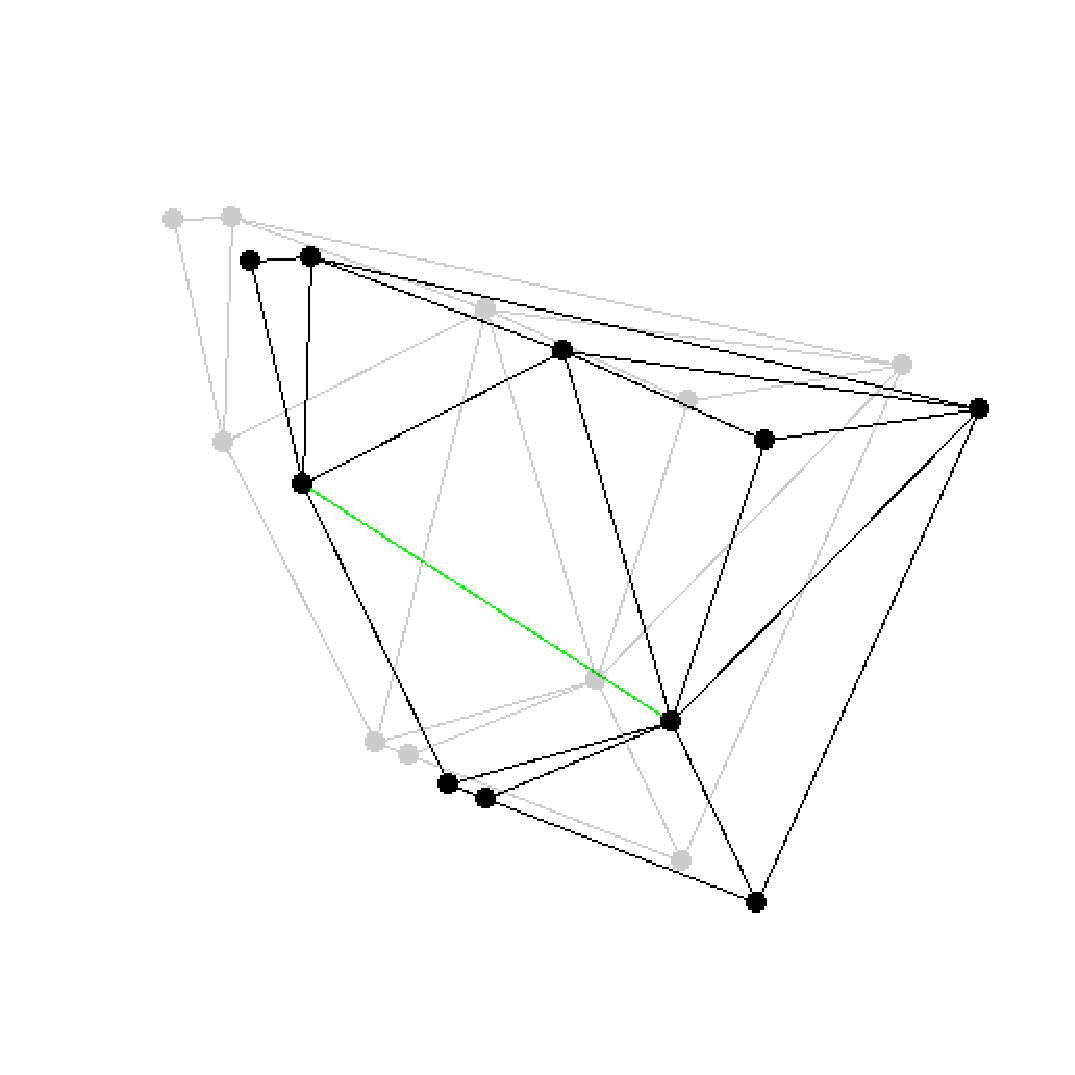
\includegraphics[ scale=.2]{Kinetic_data_structures/delaunay_7}
9.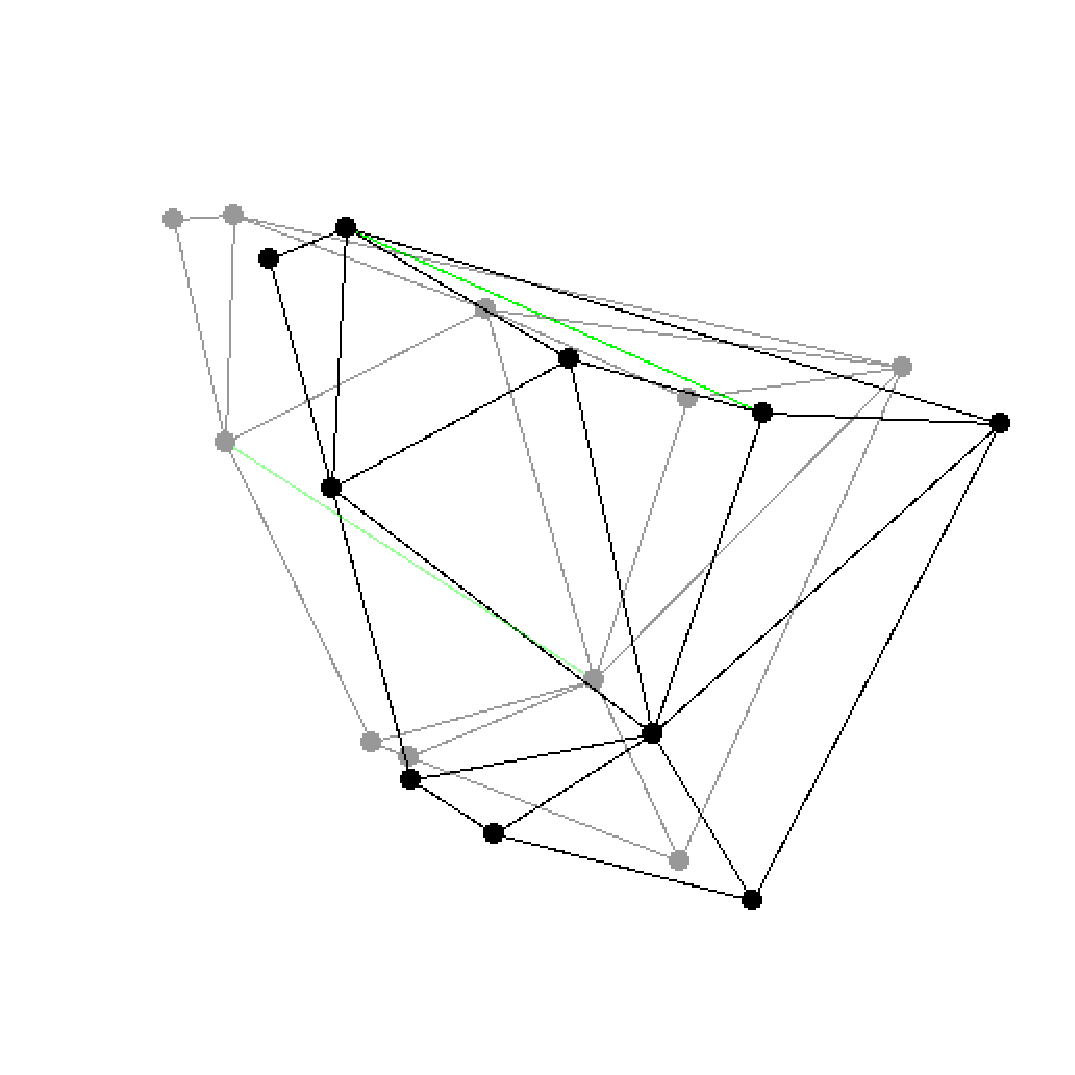
\includegraphics[ scale=.2]{Kinetic_data_structures/delaunay_8}
\end{center}
\end{ccTexOnly}
%width=300 height=300
\begin{ccHtmlOnly}

<img border=1 src="./delaunay_0.gif" align=middle alt="Frame 0" >
<img border=1 src="./delaunay_1.gif" align=middle alt="Frame 1" >
<img border=1 src="./delaunay_2.gif" align=middle alt="Frame 2" >
<img border=1 src="./delaunay_3.gif" align=middle alt="Frame 3" >
<img border=1 src="./delaunay_4.gif" align=middle alt="Frame 4" >
<img border=1 src="./delaunay_5.gif" align=middle alt="Frame 5" >
<img border=1 src="./delaunay_6.gif" align=middle alt="Frame 6" >
<img border=1 src="./delaunay_7.gif" align=middle alt="Frame 7" >
<img border=1 src="./delaunay_8.gif" align=middle alt="Frame 8" >
<br>
\end{ccHtmlOnly}
\caption{ \label{fig:kds_delaunay_events} 
{\em Some events from a Delaunay triangulation kinetic data
structure:} The state of the two dimensional Delaunay triangulation
immediately following the first events is shown. Green edges are ones
which were just created. The pictures are screen shots from
\ccc{demo/Kinetic\_data\_structures/Kinetic\_Delaunay\_triangulation\_2.cpp}. }
%\end{minipage}
%\end{center}
\end{figure*}


\begin{figure}
\begin{ccTexOnly}
\begin{center}
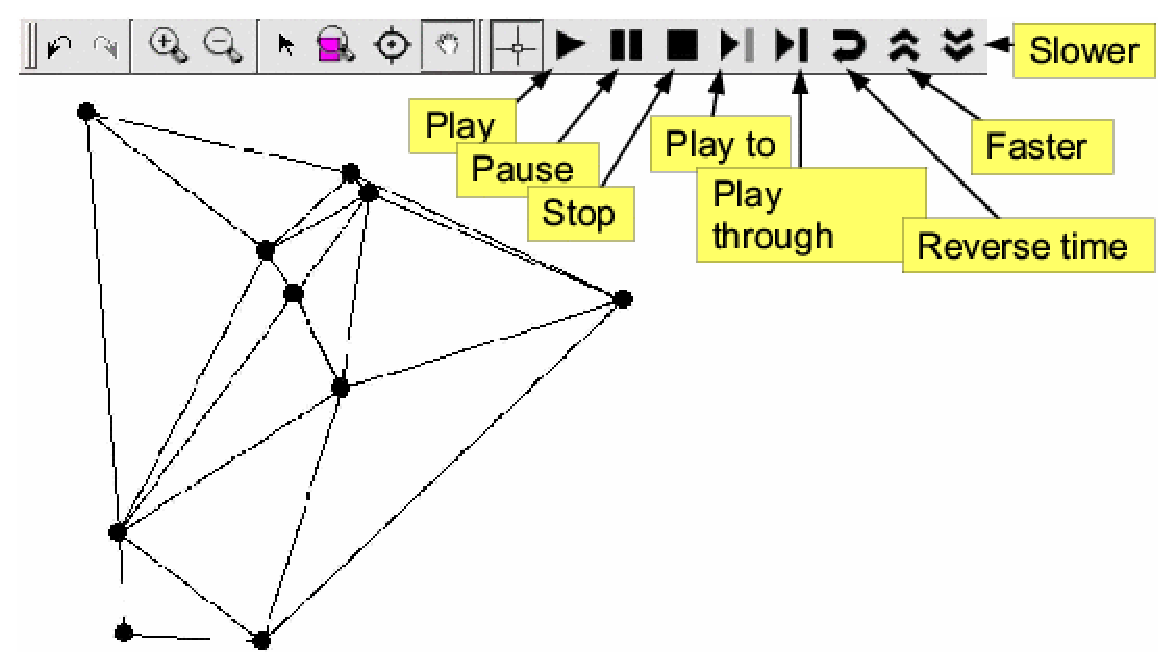
\includegraphics[scale=.5]{Kinetic_data_structures/qt_widget_marked_pct}
\end{center}
\end{ccTexOnly}
\begin{ccHtmlOnly}
<img src="./qt_widget_marked_pct.gif" align=middle alt="Qt widget"> <br>
\end{ccHtmlOnly}
\caption{\label{fig:kds_qtwidget_capture} The figure shows the graphical user interface for
  controlling two-dimensional kinetic data structures. It is built on
  top of the \ccc{Qt_widget} and adds buttons to play, pause, step
  through and run the simulation backwards.}
\end{figure}




\subsection{A Sweepline Algorithm}
\label{sec:sweepline_example}

Here we present a simple example that uses the kinetic data structures
framework to implement a sweepline to compute the arrangement of
x-monotone algebraic curves in the plane. The example builds on top of
the \ccc{Kinetic::Sort<Traits, Visitor>} kinetic data structure, using a visitor
to keep track of changes to the sorted order and newly inserted
points. To see an example using this kinetic data structure read the
example at examples/Kinetic\_data\_structures/sweepline.C.

First we define the visitor class. An object of this type is passed to
the \ccc{Kinetic::Sort} data structure and turns events into calls on
the arrangement structure. This class has to be handled externally
since the arrangement will inherit from the sorting structure.

\begin{ccExampleCode}
template <class Arrangement>
struct Arrangement_visitor: public \ccc{Kinetic::Sort}_visitor_base
{
  Arrangement_visitor(Arrangement *a):p_(a){}
  template <class Vertex_handle>
  void remove_vertex(Vertex_handle a) {
    p_->erase(a);
  }
  template <class Vertex_handle>
  void create_vertex(Vertex_handle a) {
    p_->insert(a);
  }
  template <class Vertex_handle>
  void after_swap(Vertex_handle a, Vertex_handle b) {
    p_->swap(a, b);
  }
  Arrangement *p_;
};

\end{ccExampleCode}

Now we define the actual kinetic data structure. 

\begin{ccExampleCode}

template <class TraitsT> 
class Planar_arrangement: 
  public \ccc{Kinetic::Sort}<TraitsT, 
			     Arrangement_visitor<Planar_arrangement<TraitsT> > > {
  typedef TraitsT Traits;
  typedef Planar_arrangement<TraitsT> This;
  typedef typename \ccc{Kinetic::Sort}<TraitsT,
				       Arrangement_visitor<This> > Sort;
  typedef Arrangement_visitor<This> Visitor;
  typedef typename Traits::Active_objects_table::Key Key;

public:
  typedef CGAL::Exact_predicates_inexact_constructions_kernel::Point_2 Approximate_point;
  typedef std::pair<int,int> Edge;
  typedef typename Sort::Vertex_handle Vertex_handle; 

  // Register this KDS with the MovingObjectTable and the Simulator
  Planar_arrangement(Traits tr): Sort(tr, Visitor(this)) {}

  Approximate_point vertex(int i) const
  {
    return approx_coords_[i];
  }

  size_t vertices_size() const
  {
    return approx_coords_.size();
  }

  typedef std::vector<Edge >::const_iterator Edges_iterator;
  Edges_iterator edges_begin() const
  {
    return edges_.begin();
  }
  Edges_iterator edges_end() const
  {
    return edges_.end();
  }

  void insert(Vertex_handle k) {
    last_points_[*k]=new_point(*k);
  }

  void swap(Vertex_handle a, Vertex_handle b) {
    int swap_point= new_point(*a);
    edges_.push_back(Edge(swap_point, last_points_[*a]));
    edges_.push_back(Edge(swap_point, last_points_[*b]));
    last_points_[*a]= swap_point;
    last_points_[*b]= swap_point;
  }

  void erase(Vertex_handle a) {
    edges_.push_back(Edge(last_points_[*a], new_point(*a)));
  }

  int new_point(typename Traits::Active_objects_table::Key k) {
    double tv= CGAL::to_double(Sort::traits().simulator_handle()->current_time());
    double dv= CGAL::to_double(Sort::traits().active_objects_table_handle()->at(k).x()(tv));
    approx_coords_.push_back(Approximate_point(tv, dv));
    return approx_coords_.size()-1;
  }

  std::vector<Approximate_point > approx_coords_;
  std::map<Key, int> last_points_;
  std::vector<Edge> edges_;

};
\end{ccExampleCode}

%%% Local Variables: 
%%% mode: latex
%%% TeX-master: t
%%% End: 



%%% Local Variables: 
%%% mode: latex
%%% TeX-master: t
%%% End: 




% LocalWords:  Guibas Menelaos CGAL templated Expr KDSs deschedule
% LocalWords:  Karavelas
